% === Begin Label Data ===
% ID: 269
% 难度星级: 
% 标签: 
% 备注: 
% 组卷引用次数: 0
% === End  Label Data ===

\begin{problem}{2026}{M}{深圳中学2026届高三二轮二阶测试}{8}{复数}
已知关于 $z$ 的方程 $(z^2-4z+5)(z^2+az+9)=0$（$a\in\mathbb{R}$）有四个互不相等的根，若这四个根在复平面上对应的点共圆，则 $a$ 的取值可能是(\hspace{1cm})
\begin{choices}
\choice{{$-4$}}
\choice{{$-6$}}
\choice{{$-7$}}
\choice{{$-9$}}
\end{choices}
\end{problem}

\begin{answer}
C
\end{answer}

\begin{solutions}
解方程 $z^2-4z+5=0$，即 $(z-2)^2 = -1 = (\pm i)^2$，解得 $z=2\pm i$.

设所对应的两点分别为 $A, B$，则 $A(2, 1), B(2, -1)$.

设 $z^2+az+9=0$ 的解所对应的两点分别为 $C, D$，记为 $C(x_1, y_1), D(x_2, y_2)$.

当 $\Delta < 0$ 时，即 $a^2-36 < 0$，解得 $-6 < a < 6$.

即当 $-6 < a < 6$ 时，因为 $A, B$ 关于 $x$ 轴对称，且 $C, D$ 关于 $x$ 轴对称，则以 $A, B, C, D$ 为顶点的四边形为矩形或等腰梯形，所以 $A, B, C, D$ 四点共圆。

此时只需 $-\dfrac{a}{2}\ne 2$，即 $a\ne-4$ 即可。 


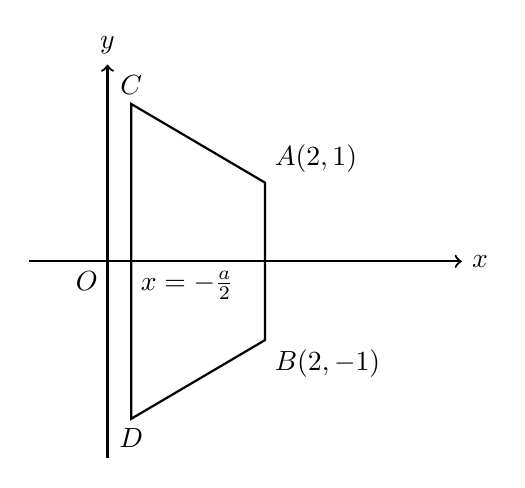
\begin{tikzpicture}[scale=1.0]
    % 绘制坐标轴
    \draw[->, thick] (-1, 0) -- (4.5, 0) node[right] {$x$};
    \draw[->, thick] (0, -2.5) -- (0, 2.5) node[above] {$y$};
    \node[below left] at (0,0) {$O$};

    % 定义点 A, B, C, D 的坐标
    % A(2,1), B(2,-1) 为 z^2-4z+5=0 的两根
    \coordinate (A) at (2, 1);
    \coordinate (B) at (2, -1);
    
    % 当 Delta < 0 时，C 和 D 是一对共轭虚根，实部相同，虚部互为相反数
    % 根据方程 z^2 + az + 9 = 0，由求根公式 z = -a/2 \pm \frac{\sqrt{36-a^2}}{2}i
    % 为了展示 C, D 不在 y 轴上的普遍情况，取 a = -2 作为示意
    % 此时实部 x = -(-2)/2 = 1，虚部 y = \pm \frac{\sqrt{36-4}}{2} = \pm \sqrt{8} \approx \pm 2.83
    % 缩放绘图比例，在图上大致取 (1, 2) 和 (1, -2)
    \coordinate (C) at (0.3, 2);
    \coordinate (D) at (0.3, -2);

    % 绘制等腰梯形 ACDB
    \draw[thick] (A) -- (C) -- (D) -- (B) -- cycle;
    
    % 绘制垂直连线 AB 和 CD
    \draw[dashed, thick] (A) -- (B);
    \draw[dashed, thick] (C) -- (D);

    % 标注 CD 所在的直线方程
    \node[below right] at (0.3, 0) {$x = -\frac{a}{2}$};

    % 标注点
    \node[above right] at (A) {$A(2,1)$};
    \node[below right] at (B) {$B(2,-1)$};
    \node[above ] at (C) {$C$};
    \node[below ] at (D) {$D$};
\end{tikzpicture}


当 $\Delta > 0$ 时，即 $a > 6$ 或 $a < -6$ 时，
此时 $C(x_1, 0), D(x_2, 0)$，且 $\dfrac{x_1+x_2}{2} = -\dfrac{a}{2}$，$x_1 x_2 = 9$.

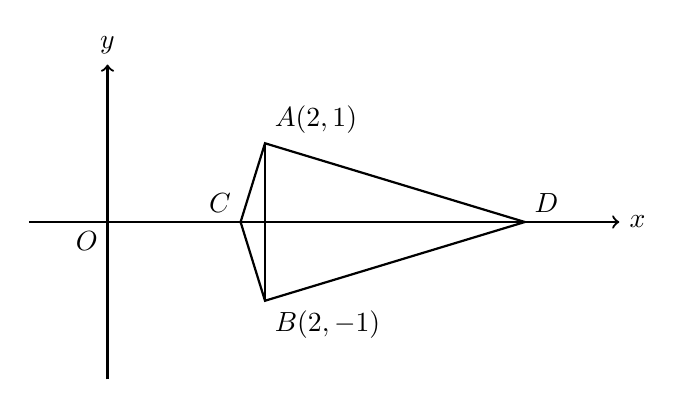
\begin{tikzpicture}[scale=1.0]
    % 绘制坐标轴
    \draw[->, thick] (-1, 0) -- (6.5, 0) node[right] {$x$};
    \draw[->, thick] (0, -2) -- (0, 2) node[above] {$y$};
    \node[below left] at (0,0) {$O$};

    % 定义点 A, B, C, D 的坐标
    % A(2,1), B(2,-1) 为 z^2-4z+5=0 的两根
    \coordinate (A) at (2, 1);
    \coordinate (B) at (2, -1);
    
    % 当 a = -7 时，z^2 - 7z + 9 = 0
    % 两个实根约为 C(1.69, 0) 和 D(5.30, 0)
    \coordinate (C) at (1.69, 0);
    \coordinate (D) at (5.30, 0);

    % 绘制四边形 ABCD
    \draw[thick] (A) -- (C) -- (B) -- (D) -- cycle;
    
    % 绘制垂直连线 AB
    \draw[thick] (A) -- (B);

    % 标注点
    \node[above right] at (A) {$A(2,1)$};
    \node[below right] at (B) {$B(2,-1)$};
    \node[above left] at (C) {$C$};
    \node[above right] at (D) {$D$};
\end{tikzpicture}



故此圆的圆心为 $O_1(-\dfrac{a}{2}, 0)$，半径
$$
r = \dfrac{|x_1-x_2|}{2} = \dfrac{\sqrt{a^2-36}}{2}.
$$

又圆心 $O_1$ 到 $A$ 的距离 $|O_1 A| = \sqrt{(2+\dfrac{a}{2})^2 + 1^2} = r$，
解得 $a = -7$.

综上可得 $a \in (-6, -4)\cup (-4,6) \cup \{-7\}$.

故答案为：$a \in (-6, -4)\cup (-4,6) \cup \{-7\}$.

结合选项，本题选 C.
\end{solutions}